% Ubah judul dan label berikut sesuai dengan yang diinginkan.
\section{Arsitektur}
\label{sec:arsitektur}

% Ubah paragraf-paragraf pada bagian ini sesuai dengan yang diinginkan.

\subsection{Perancangan Sistem Deteksi Helm Keselamatan Kerja}
\label{subsec:perancangansistemdeteksihelmkeselamatankerja}

\par This hardhat detection system will utilize YOLOv5 to make 
predictions on the input received. Input is an image received from a 
webcam or camera connected to a computer that will run this system. 
The system was developed with the aim of detecting the use of work 
safety helmets in real-time and will run an alarm mechanism if on the 
camera input there is someone who is not wearing a work safety helmet. 
The flowchart for the Safety Helmet Detection system can be seen at Figure~\ref{fig:flowchart_sistem}.


\par The system will be created as a python script file that can be run and can accept several parameters: 
input source, weight to be used, confidence threshold, and IoU threshold for the Non Max Suppression process.
\par Input that can be used with the created script can be done in the form of video files or camera feeds.
The system can accept various resolutions, but for the inference process, the input dimensions will 
be resized to 640x640 and the output will be adjusted to the dimensions of the initial input.

\par Each frame that comes in from the input webcam will be used to process inference via
yolov5 model with weight that has been created previously through the training process.
The result of inference using YOLOv5 will return the input in the form of position for
the detected object is in xcenter, ycenter and the dimension of the object is in widht
and height as well as the name information class and confidence score for
each detected object. The result of output inference obtained is then used to draw
bounding box on the frame image being inference
as in Figure~\ref{fig:outputboundingbox}.

% Contoh input gambar pada kolom.
\begin{figure} [ht]
  \centering
  % Ubah sesuai dengan nama file gambar dan ukuran yang akan digunakan.
  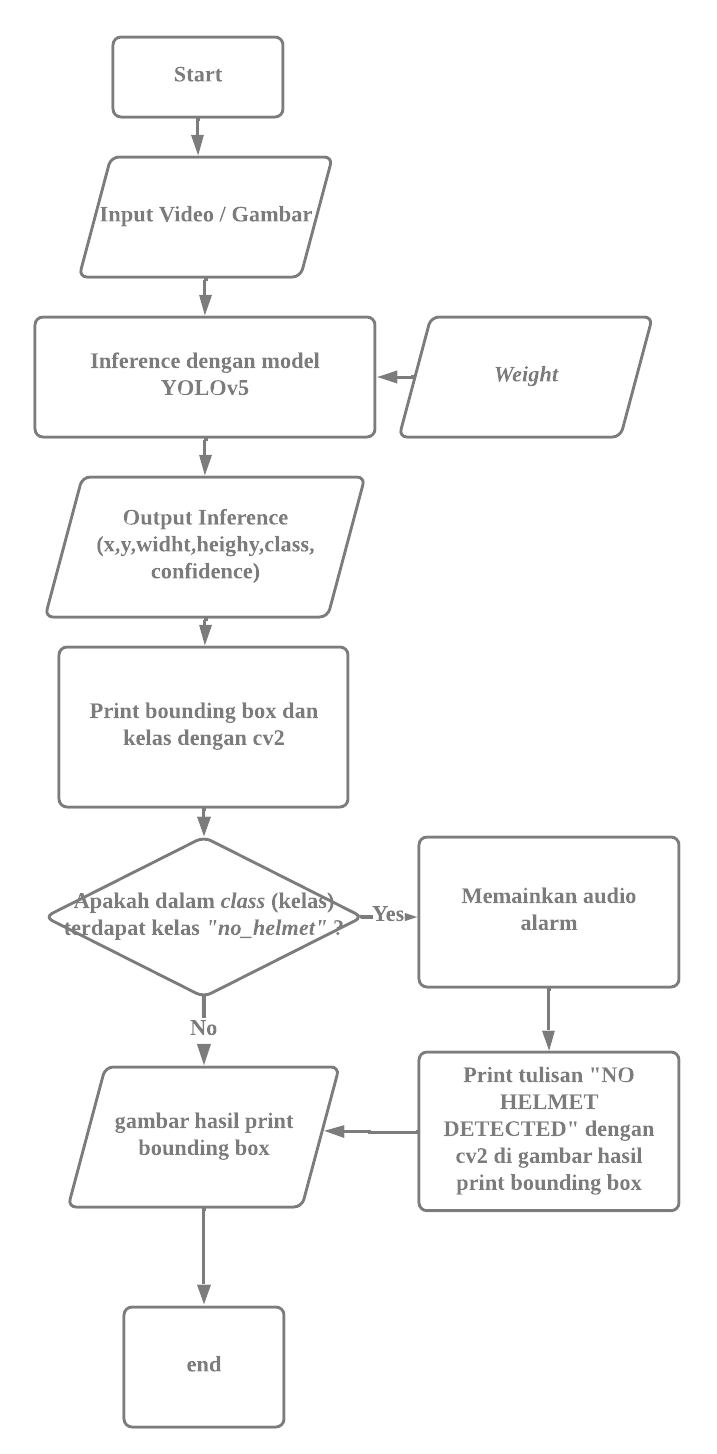
\includegraphics[width=0.4\textwidth]{gambar/flowchart_sistem.png}

  % Ubah sesuai dengan keterangan gambar yang diinginkan.
  \caption{flowchart Sistem}
  \label{fig:flowchart_sistem}
\end{figure}

\subsection{Model YOLOv5}
\label{subsec:yolov5model}

YOLOv5 merupakan versi pembaruan dari YOLO yang dicetuskan pada tahun 2020 oleh Glenn Jocher \cite{glenn_jocher_yolov5}. Berdasarkan dari \emph{repository} Github untuk YOLOv5 oleh Glenn Jocher, struktur jaringan dari YOLOv5 dibagi menjadi 3 bagian utama yaitu modul \emph{Backbone}, \emph{Neck}, dan \emph{Head}.
Seperti yang dapat dilihat di Gambar \ref{fig:yolov5network} Struktur jaringan dari YOLOv5 ini dimulai dari modul \emph{Backbone} dimana dilewati pertama oleh input gambar untuk mengekstrak fitur - fitur dari gambar yang strukturnya berbasis dari struktur \emph{Focus}, \emph{Bottleneck CSP (Cross Stage Partinal Networks)}, dan \emph{Spatial Pyramid Pooling (SPP)}.
Hasil ekstraksi fitur dari \emph{Backbone} lalu digunakan untuk menghasilkan \emph{feature pyramid} di modul \emph{Neck} yang merupakan struktur yang berbasis dari PANet (\emph{Path Aggregation Network}).
Lalu terakhir di Modul \emph{Head} dilakukan penampilan \emph{bounding box} yang meliputi beberapa informasi yaitu : kelas, koordinat, dan \emph{confidence score}.

\begin{figure} [ht]
  \centering
  % Ubah sesuai dengan nama file gambar dan ukuran yang akan digunakan.
  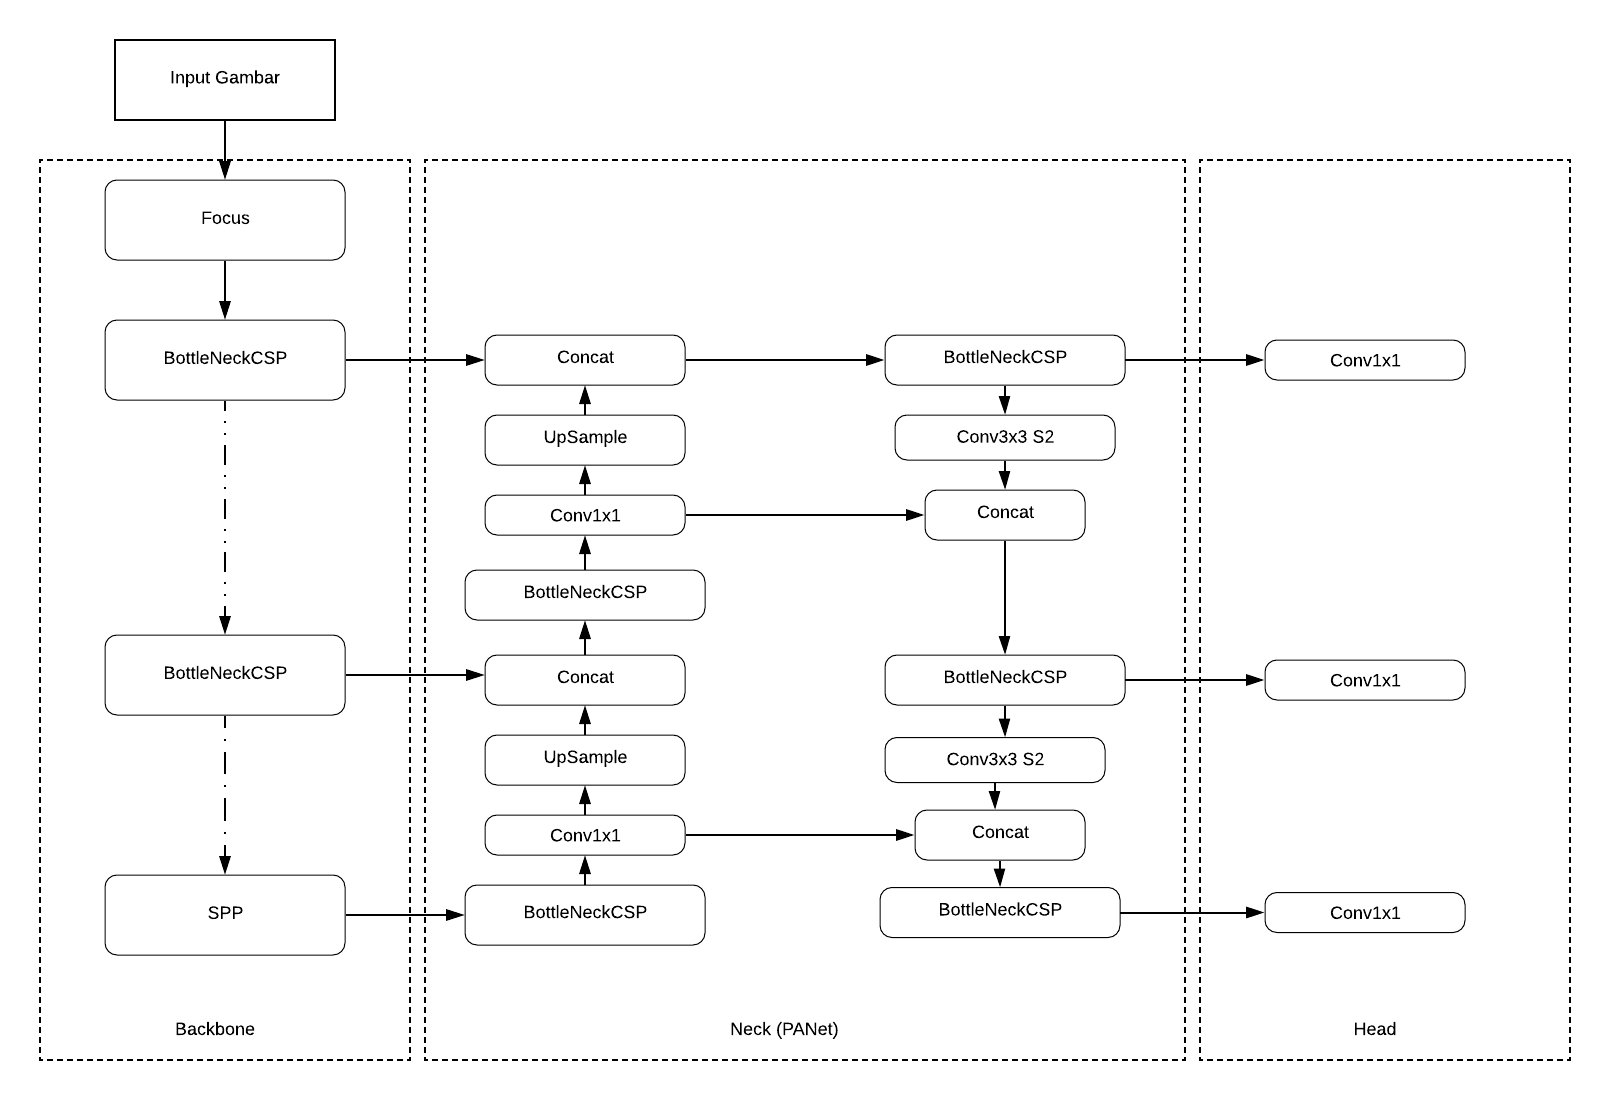
\includegraphics[width=0.4\textwidth]{gambar/yolov5 structure.png}

  % Ubah sesuai dengan keterangan gambar yang diinginkan.
  \caption{YOlov5}
  \label{fig:yolov5s}
\end{figure}

% Contoh pembuatan tabel.
\begin{table}
  \caption{Contoh tabel sederhana}
  \label{tab:tabelsederhana}
  \centering
  \begin{tabular}{lll}
    \toprule
    Heading1 & Heading2 & Heading3  \\
    \midrule
    One      & Two      & Three     \\
    Four     & Five     & Six       \\
    \bottomrule
  \end{tabular}
\end{table}

% Contoh pembuatan potongan kode.
\begin{lstlisting}[
  language=C++,
  caption={Program halo dunia.},
  label={lst:halodunia}
]
#include <iostream>

int main() {
    std::cout << "Halo Dunia!";
    return 0;
}
\end{lstlisting}

\lipsum[12]

% Contoh pembuatan daftar.
\begin{enumerate}
  \item \lipsum[13][1-4]
  \item \lipsum[13][5-8]
  \item \lipsum[13][9-12]
\end{enumerate}

\lipsum[14-15]
